
\subsection{link-analysis}

There are two parameters to \textit{link-analysis}: $\gamma$ and $\eta$. They are both continuous and both are undefined at 0.

The following plot is evaluated using \textit{F-measure} w.r.t. the test set using top-10 recommendations over the parameter space of both $\gamma$ and $\eta$.

\begin{figure}[h!]
    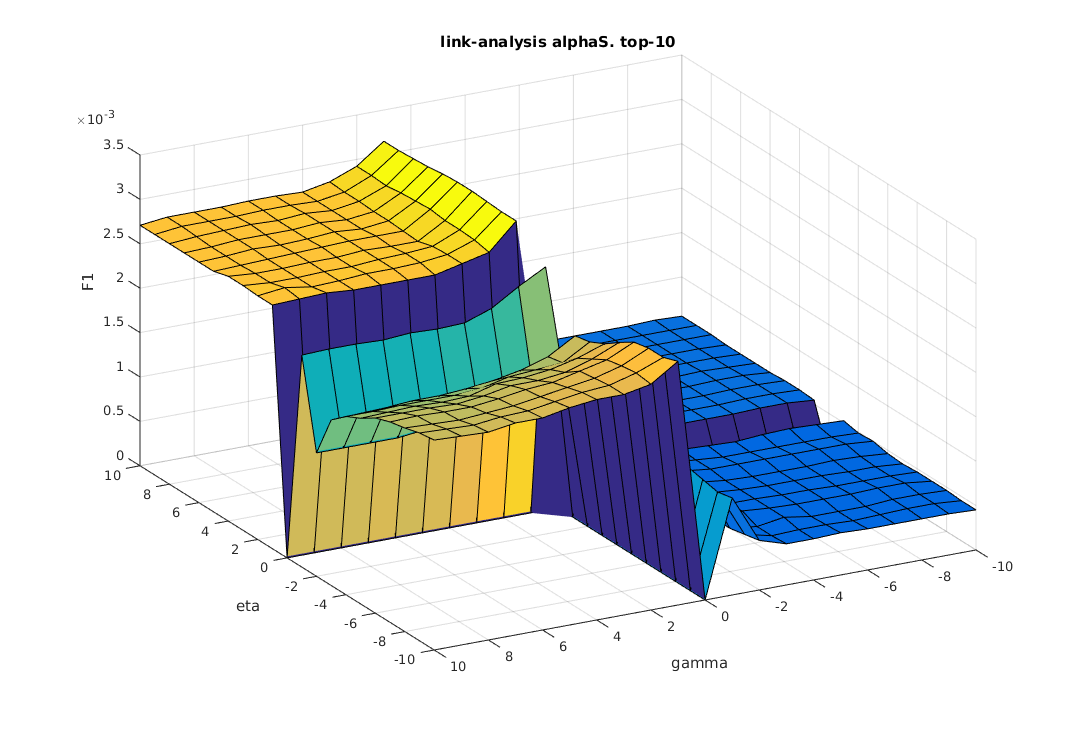
\includegraphics[width=\textwidth]{fig/link_eta_gamma/alphaS_link_eta.png}
    \caption{\textit{alphaS}}
    \label{fig:linkalphaS}
\end{figure}

As noted before, the function is undefined at $\gamma = 0$ and $\eta = 0$. For \textit{alphaS} it appears $\gamma < 0$ is a very bad choice. Both $\eta > 0$ and $\eta < 0$ seems to be fair choices.

\begin{figure}[h!]
\centering
\begin{minipage}{.5\textwidth}
    \centering
    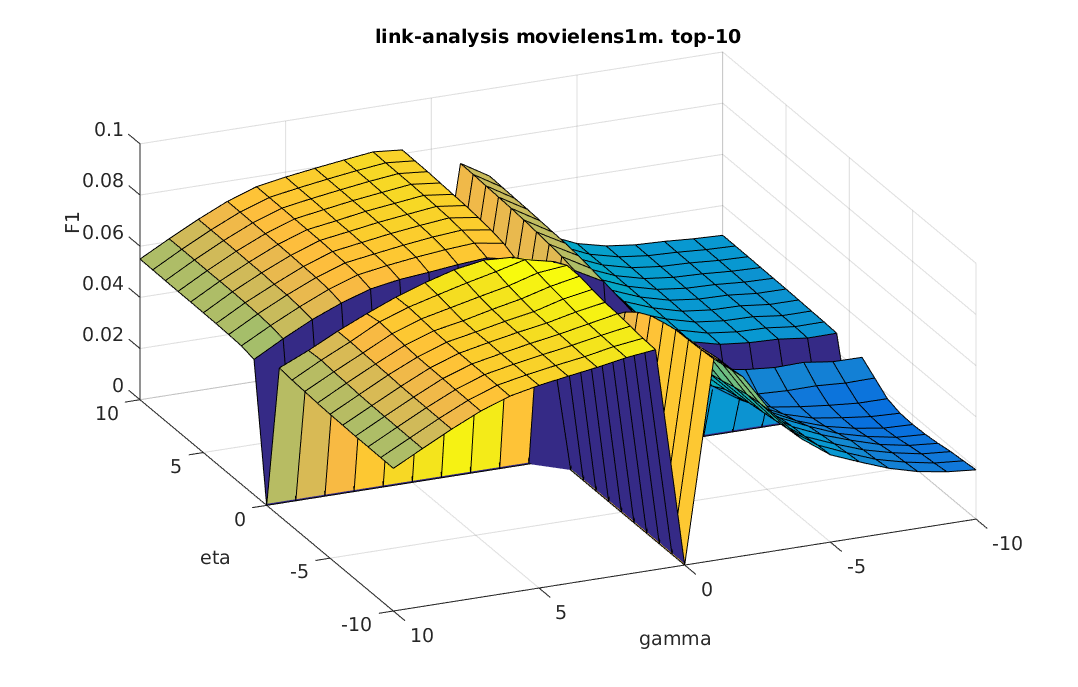
\includegraphics[width=\linewidth]{fig/link_eta_gamma/movielens_link_eta.png}
    \captionof{figure}{\textit{movielens1m}}
\end{minipage}%
\begin{minipage}{.5\textwidth}
    \centering
    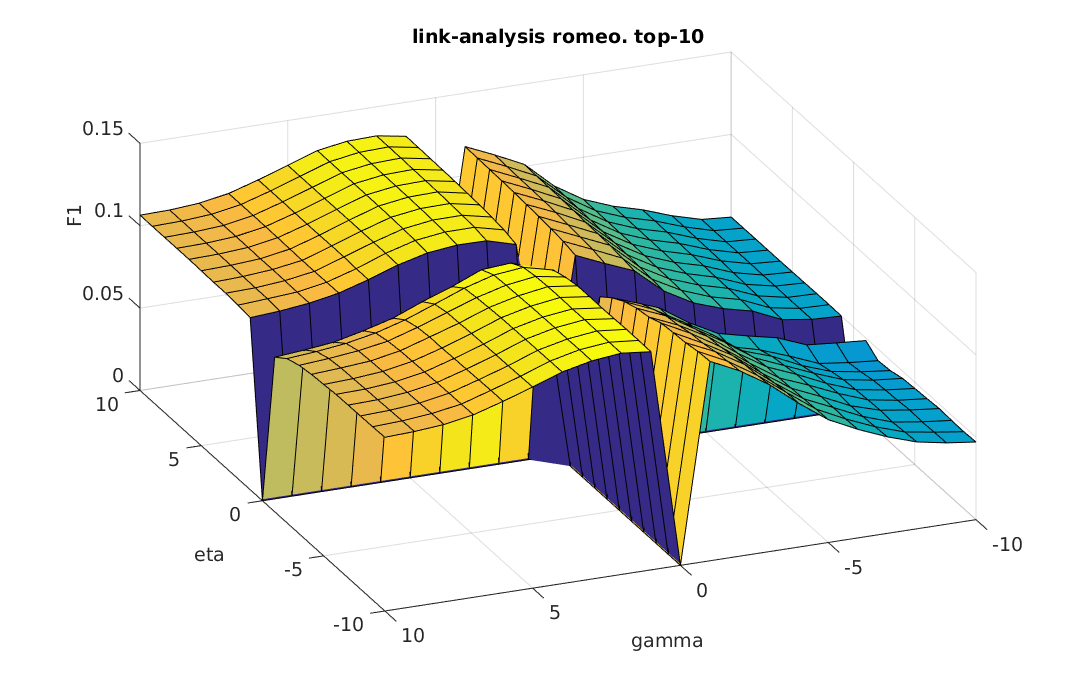
\includegraphics[width=\linewidth]{fig/link_eta_gamma/romeo_link_eta.png}
    \captionof{figure}{\textit{romeo}}
\end{minipage}
\end{figure}

Similar observations can be made for \textit{movielens1m} and \textit{romeo}. The function space seems to be fairly smooth, almost convex. \textit{alphaS} has an anomaly at $\eta = -2$ and the parameters at 0 are exceptions.

\FloatBarrier

\begin{figure}[h!]
    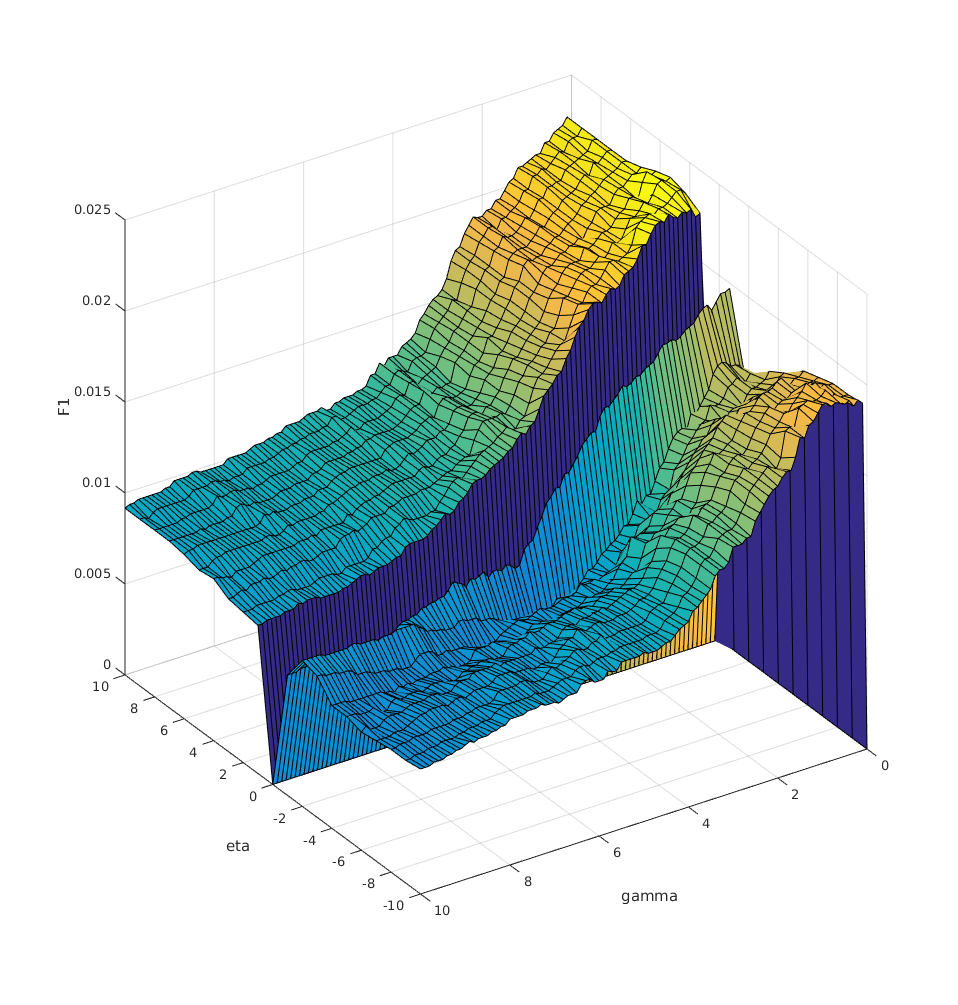
\includegraphics[width=\textwidth]{fig/link_eta_gamma/eswc2015books.png}
    \caption{\textit{eswc2015books}}
\end{figure}

\FloatBarrier

A closer look at \textit{eswc2015books}, ignoring $\gamma < 0$, reveals that the function space isn't as smooth as it might have seemed in the previous plots, several local optima can be seen. An anomaly around $\eta = -2$ is visible here as well.

\newpage

Interestingly some of the datasets have their maximum at $\eta > 0$ but others have $\eta < 0$. What follows is some plots over $\eta$ and a fixed $\gamma = 2$.

\FloatBarrier

\begin{figure}[h!]
\centering
\begin{minipage}{.5\textwidth}
    \centering
    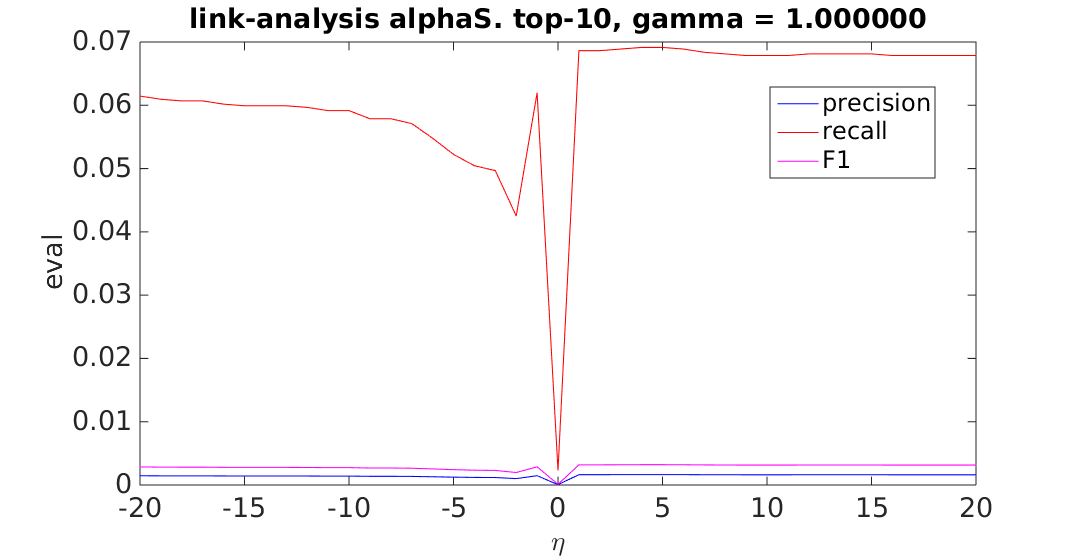
\includegraphics[width=\linewidth]{fig/link_eta/alphaS_link_eta.png}
    \captionof{figure}{\textit{alphaS}}
\end{minipage}%
\begin{minipage}{.5\textwidth}
    \centering
    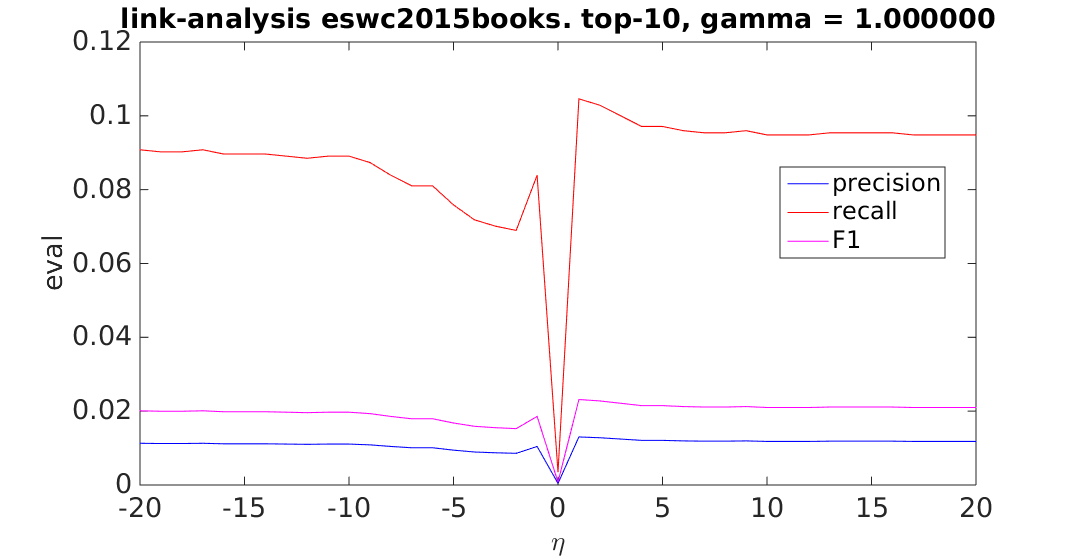
\includegraphics[width=\linewidth]{fig/link_eta/eswc2015books_link_eta.png}
    \captionof{figure}{\textit{eswc2015books}}
\end{minipage}
\end{figure}

\begin{figure}[h!]
\centering
\begin{minipage}{.5\textwidth}
    \centering
    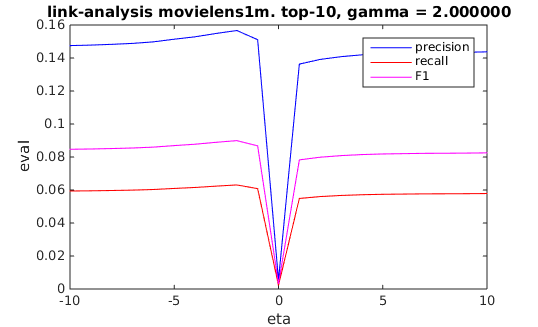
\includegraphics[width=\linewidth]{fig/link_eta/movielens_link_eta.png}
    \captionof{figure}{\textit{movielens1m}}
\end{minipage}%
\begin{minipage}{.5\textwidth}
    \centering
    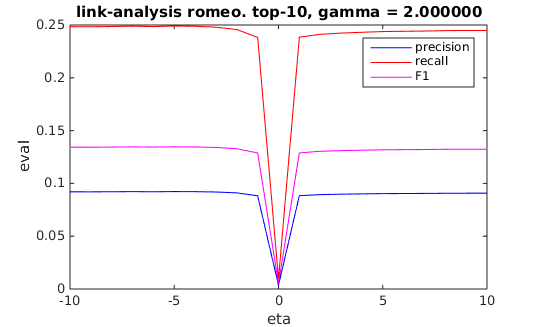
\includegraphics[width=\linewidth]{fig/link_eta/romeo_link_eta.png}
    \captionof{figure}{\textit{romeo}}
\end{minipage}
\end{figure}

\FloatBarrier

Here \textit{alphaS} and \textit{eswc2015books} have maximum \textit{F-measure} with $\eta < 0$ but \textit{movielens1m} and \textit{romeo} with $\eta > 0$.

The actual optima, given optimization criteria of $\eta$ and $\gamma$, can be different. As can be seen in \figureref{fig:linkalphaS} the optima uses a smaller $\gamma$ and a positive $\eta$. But the local optima can still be found with either $\eta > 0$ or $\eta < 0$.

\newpage

$\gamma$ is the parameter which seems to vary the function value the most. The following plots varies $\gamma$ while holding $\eta = 1$ constant.

\FloatBarrier

\begin{figure}[h!]
\centering
\begin{minipage}{.5\textwidth}
    \centering
    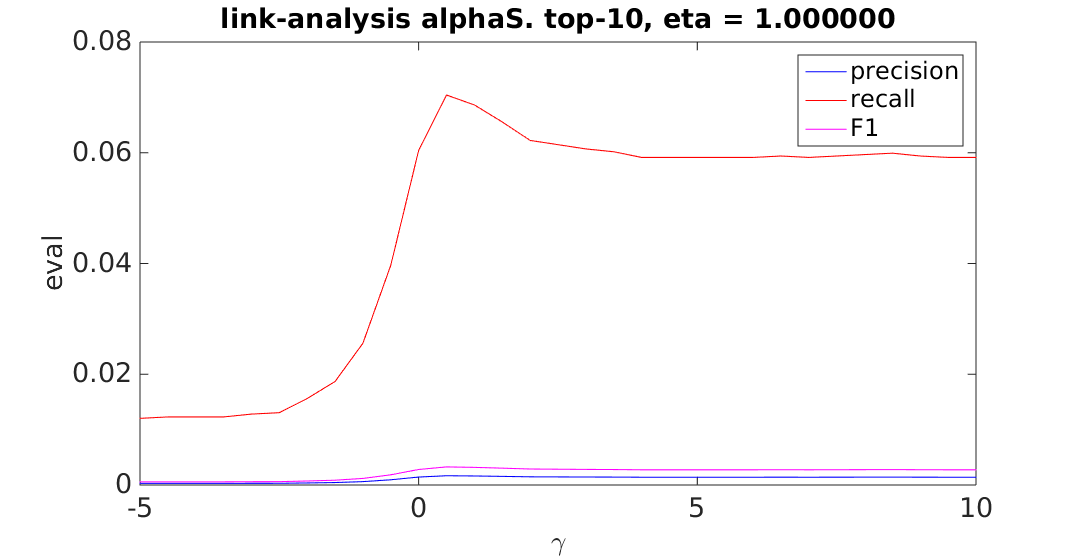
\includegraphics[width=\linewidth]{fig/link_gamma/alphaS_link_gamma.png}
    \captionof{figure}{\textit{alphaS}}
\end{minipage}%
\begin{minipage}{.5\textwidth}
    \centering
    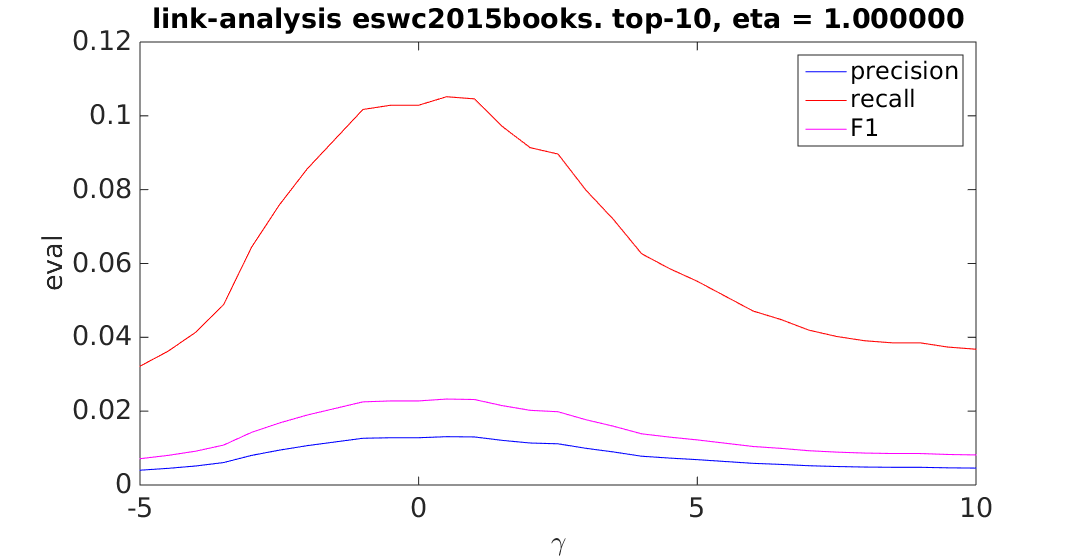
\includegraphics[width=\linewidth]{fig/link_gamma/eswc2015books_link_gamma.png}
    \captionof{figure}{\textit{eswc2015books}}
\end{minipage}
\end{figure}

\begin{figure}[h!]
\centering
\begin{minipage}{.5\textwidth}
    \centering
    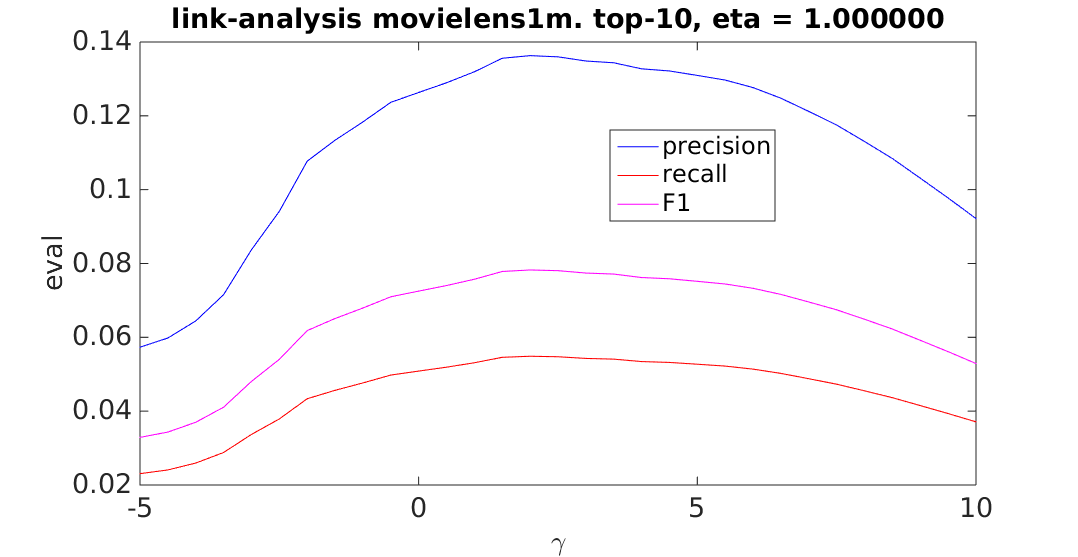
\includegraphics[width=\linewidth]{fig/link_gamma/movielens_link_gamma.png}
    \captionof{figure}{\textit{movielens1m}}
\end{minipage}%
\begin{minipage}{.5\textwidth}
    \centering
    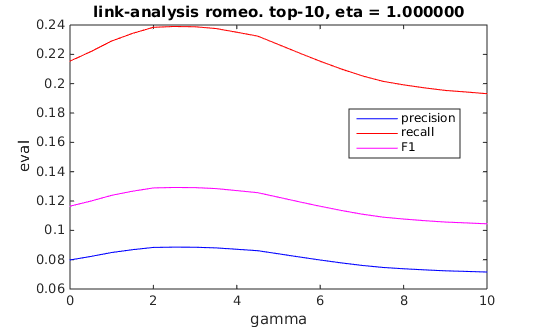
\includegraphics[width=\linewidth]{fig/link_gamma/romeo_link_gamma.png}
    \captionof{figure}{\textit{romeo}}
\end{minipage}
\end{figure}

\FloatBarrier
